\documentclass[12pt, titlepage]{article}
%------------------------------------------------------------

% Packages --------------------------------------------------
%Kopf und Fusszeile
\usepackage[headsepline]{scrpage2}
%Dokumentsabmessung
\usepackage[left=3cm,top=2.5cm,right=3cm,bottom=2.5cm]{geometry}
\usepackage[utf8]{inputenc}
\usepackage[T1]{fontenc}
\usepackage{lmodern}
\usepackage[german]{babel}
\usepackage{microtype} %verbessert Darstellung

%Abkürzungsverzeichnis
\usepackage[nohyperlinks, printonlyused]{acronym}

\usepackage[nottoc]{tocbibind}

\usepackage{graphicx}
\usepackage{float}
\usepackage{subfig}
\usepackage{ragged2e}

\usepackage{hyperref}
%\usepackage{natbib} Harvard-Style
\usepackage[authoryear]{natbib}
\bibliographystyle{dcu}
%plainnat
%dcu
\usepackage{enumitem}

%\usepackage[author={Manu},markup=StrikeOut,color=red]{pdfcomment}

\usepackage[rgb]{xcolor}

\normalsize

%Querformatseiten
\usepackage{pdflscape}
%nur Text im Querformat
%\usepackage{lscape}

%Abbildung im Verzeichnis verhindern
\usepackage{caption}
%\usepackage[onehalfspacing]{setspace}

%Tabellen
\usepackage{tabularx}
\usepackage{array}
\usepackage{booktabs}
\usepackage{siunitx}
\usepackage{color, colortbl}

%Regressionstabellen aus Stata sauber importieren
\usepackage{dcolumn}
%\usepackage{multicol}

%Zentrierte Tabellen über Komma
\usepackage{multirow}

%Gesplittete Gleichungen
\usepackage{amsmath}
\usepackage{amsthm}
\usepackage{amsbsy}
\usepackage{amssymb}
\usepackage{textcomp}
\usepackage{wasysym}
\numberwithin{equation}{section} %Nummeriert die Formeln nach Kapitel
\usepackage{siunitx}


%Fussnoten bei Tabelle
\usepackage{setspace}
\usepackage{threeparttable}

%Kopf und Fusszeile
\usepackage{scrpage2}
\renewcommand{\headfont}{\scriptsize}
\pagestyle{scrheadings}
\clearscrheadfoot
\chead{O9 Interferenz und Beugung}
\ofoot{\normalsize\pagemark}
\setheadsepline{.4pt}
\setfootsepline{.4pt}
\cfoot{Simon Zoller, Elias von Däniken}

%Fett und kleinere Schrift bei Beschriftungen
\usepackage[labelfont={bf,sf},font={footnotesize},
labelsep=colon]{caption}

%Zeigt im Inhaltsverzeichniss nur section und subsection an
\setcounter{tocdepth}{2} 
\setcounter{secnumdepth}{3} 
%------------------------------------------------------------

%Zeilen einrücken verhindern
\setlength{\parindent}{0em}

% Dokument --------------------------------------------------
\begin{document}

% Titelseite -----------------------------------------------------
\begin{titlepage}
	
\end{titlepage}

%------------------------------------------------------------


% Inhaltsverzeichnis ----------------------------------------
\pagenumbering{Roman}
\tableofcontents

%\newpage
%\listoffigures% Abbildungsverzeichnis
%\newpage
%\listoftables% Tabellenverzeichnis
%\newpage
%\phantomsection \addcontentsline{toc}{section}{Abkürzungsverzeichnis}
\newpage



% Inhalt ------------------------------------------------------
\pagenumbering{arabic}  

% Kapitel 1----------------------------------------------------
% Kapitel 1 Arbeitsgrundlagen------------------------------------------------- %
\section{Arbeitsgrundlagen}
% ---------------------------------------------------------------------------- %
In diesem Abschnitt werden die Arbeitsgrundlagen zur Beugung und Interferenz für den Versuch erarbeitet.
% **************************************************************************** %
\subsection{Huygenssches Prinzip}
% **************************************************************************** %
Das huygensche Prinzip besagt, dass jeder Punkt einer Wellenfläche als Ausgangspunkt einer Elementarwelle betrachtet werden kann, die sich mit gleicher Phasengeschwindigkeit und Wellenlänge wie die ursprüngliche Welle ausbreitet. Durch die Überlagerung sämtlicher Elementarwellen ergibt sich die neue Lage der Wellenfront. Es bildet sich eine rücklaufende Welle, da die Elementarwelle eine Kugelform hat.

\begin{figure}[h!]
	\centering
	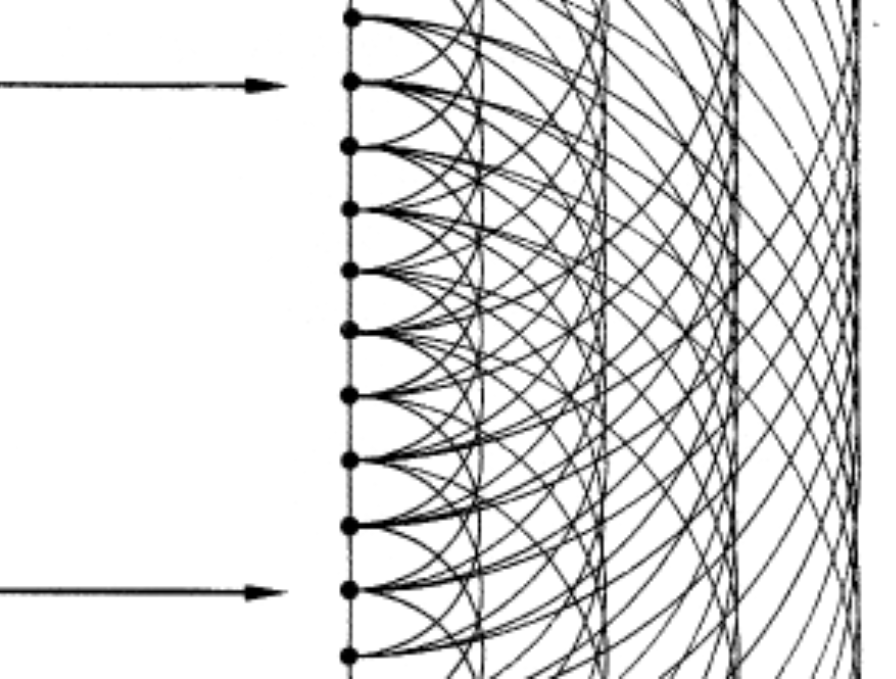
\includegraphics[width=0.8\textwidth]{data/huygens}
	\caption{Eine Welle die sich aus Überlagerungen von Kugelwellen bildet. Mit den schwarzen Punkten sind die Punkte, welcher von einer Wellenfront erreicht wird, dargestellt. Dies ist der Ausgangspunkt für eine kugelförmige Elementarwelle. }
	\label{fig:heygens}
\end{figure}
\newpage

In Abbildung \ref{fig:heygens_spalt} wird das huygensche Prinzip auf die Beugung von Licht an Hindernissen angewandt. Eine ebene Wellenfront wird an einem Spalt gebeugt. Es entsteht näherungsweise eine Rechtecksform. Nach dem Prinzip der Interferenz kann die resultierende Welle durch Superposition aller Elementarwellen berechnen lässt. 

\begin{figure}[h!]
	\centering
	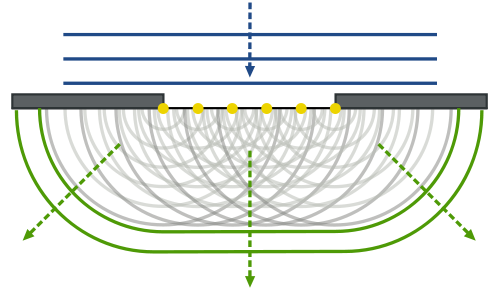
\includegraphics[width=0.8\textwidth]{data/hspalt.png}
	\caption{Beugung einer ebenen Wellenfront an einem Spalt nach dem huygensschen Prinzip.}
	\label{fig:heygens_spalt}
\end{figure}



%https://de.wikipedia.org/wiki/Huygenssches_Prinzip

%http://www.dieter-heidorn.de/Physik/SS/K03_Wellen/K03_Huygens/K03_Huygens.html

\newpage
% **************************************************************************** %
\subsection{Beugungsintegral}
% **************************************************************************** %
Die Beugung von Licht an eine beliebig geformte Blende kann mit dem Beugungsintegral berechnet werden. Dieses Beugungsintegral basiert auf dem Modell der Elementarwellen. Für das Beugungsintegral gibt es zwei Näherungen. Für das Nahfeld wird die Fresnel-Näherung und für das Fernfeld die Fraunhofer-Näherung angewandt. Das System, welches mit mittels Kirchhoffischen Beugungsintegral beschrieben wird skizziert. Die Formel \ref{eq:integral} beschreibt wie man die Amplitude $ \phi_{P} $ im Punkt P auf dem Beobachtungsschirm berechnet werden kann. Die Berechnung ist Abhängig von der Amplitude der Quelle $ a_{Q} $, dem Betrag des Wellenvektors in der Quelle $ k_{0} = 2 \pi/\lambda $, der Wellenlänge $ \lambda $, den Neigungsfaktoren $ \theta $ und $ \theta_{1} $, den Abständen $ L $, $ L_{1} $, $ d $, $ d_{1} $ und der Blendfunktion $ f(s) $. Bei einer vollkommenen undurchlässigen Blende beträgt die Blendfunktion $ f(s)=0 $ und bei einer vollkommen durchlässigen Blende beträgt $ f(s)=1 $.

\begin{equation}\label{eq:integral}
\psi_{p}=\frac{a_{Q}\cdot k_{0}}{2\cdot \pi \cdot i} \int_{Blende} f(s) \cdot\frac{e^{i\cdot k_{0}\cdot (d +d_{i})}}{d\cdot d_{1}} \cdot \left[ \frac{cos\theta + cos\theta_{1}}{2} \right] ds
\end{equation}

\begin{figure}[h!]
	\centering
	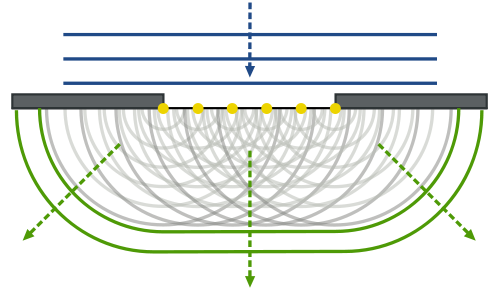
\includegraphics[width=0.8\textwidth]{data/hspalt.png}
	\caption{Die Anordnung besteht aus einer Lichtquelle $ Q $, einer Blende $ S $, an der das Licht gebeugt wird und einem Beobachtungsschirm auf dem die auftreffende Lichtintensität an P untersucht wird.}
	\label{fig:integral}
\end{figure}

% **************************************************************************** %
\subsection{Frauenhofer-Näherung}
% **************************************************************************** %
Die Fernfeld-Näherung des Beugungsintegral (Formel \ref{eq:integral}) entspricht die Frauenhofer-Näherung. Bei dieser Näherung wird angenommen, dass . Der Term mit den Neigungsfaktoren $ \theta $ und $ \theta_{1} $ kann in diesem Fall vernachlässigt werden. Zudem lässt sich wegen dieser Näherung $ d\cdot d_{1} $ im Nenner durch $ L\cdot L_{1} $ ersetzt. Der Ausdruck $ d + d_{1} $ im Exponent enthält die Information zur Phase, deshalb darf hier nicht $ d $ durch $ L $ ersetzt werden. Sie können jedoch mit einer Taylor-Reihe  vereinfacht werden. 


\subsubsection{Frauenhofer'sche Beobachtungsart}
Bei der Frauenhofer'sche Beobachtungsart wird das Interfernzmuster, wie in der Abbildung \ref{fig:beobachtungsart} dargestellt, in der Brennebene beobachtet. Dies geschieht in dem das Interferenzmuster durch eine Linse auf einen Schirm projiziert wird. Die Linse wird im Abstand $ f $ vor dem Schirm platziert. Das beobachtete Muster ist bis auf einen Skalierungsfaktor identisch zum Interferenzmuster, welches in grosser Entfernung von den Quellen beobachtet werden kann. Der Abstand von der Linse von den Quellen hat keinen Einfluss auf die Abmessung oder die Form des Interferenzmuster. Er bestimmt nur den erfassten Winkelbereich.

\begin{figure}[h!]
	\centering
	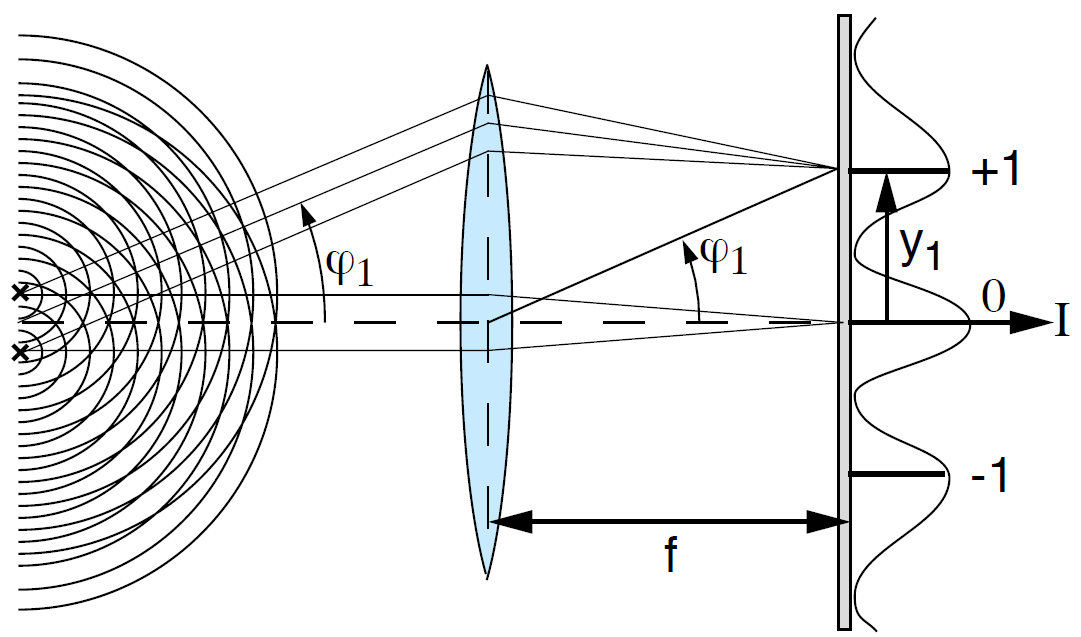
\includegraphics[width=0.8\textwidth]{data/fraunhofer}
	\caption{Frauenhofer'sche Beobachtungsart}
	\label{fig:beobachtungsart}
\end{figure}

Der Winkel $ \phi_{1} $ der Interferenz erster Ordnung kann mit dem Abstand $ y_{1} $ von dem Hauptstrahl zum Extrema der ersten Ordnung und der Brennweite $ f $ der Linse wie folgt berechnen.
\begin{equation}\label{eq:frauenhofer}
tan(\phi_{1}) =  \frac{y_{1}}{f}
\end{equation}

\newpage
% Kapitel 2----------------------------------------------------
% Kapitel 2 Arbeitsmittel------------------------------------------------- %
\section{Arbeitsmittel}
% ---------------------------------------------------------------------------- %
In diesem Kapitel wird der Versuchsaufbau, die Messmittel und der Messvorgang genauer erläutert.

% **************************************************************************** %
\subsection{Versuchsaufbau}
% **************************************************************************** %
Der Versuchsaufbau, wie in der Abbildung \ref{fig:Versuchsaufbau} aufgezeigt, beseht aus der Lichtquelle, dem zu messende Beugungsobjekt und einer Linse, welche auf einer Zeiss-Schiene montiert sind. Das zu beobachtenden Beugungsmuster kann am Ende der Schiene mit einer Messeinrichtung gemessen werden. Die Messeinrichtung ist auf einer Mattscheibe montiert.

\begin{figure}[h!]
	\centering
	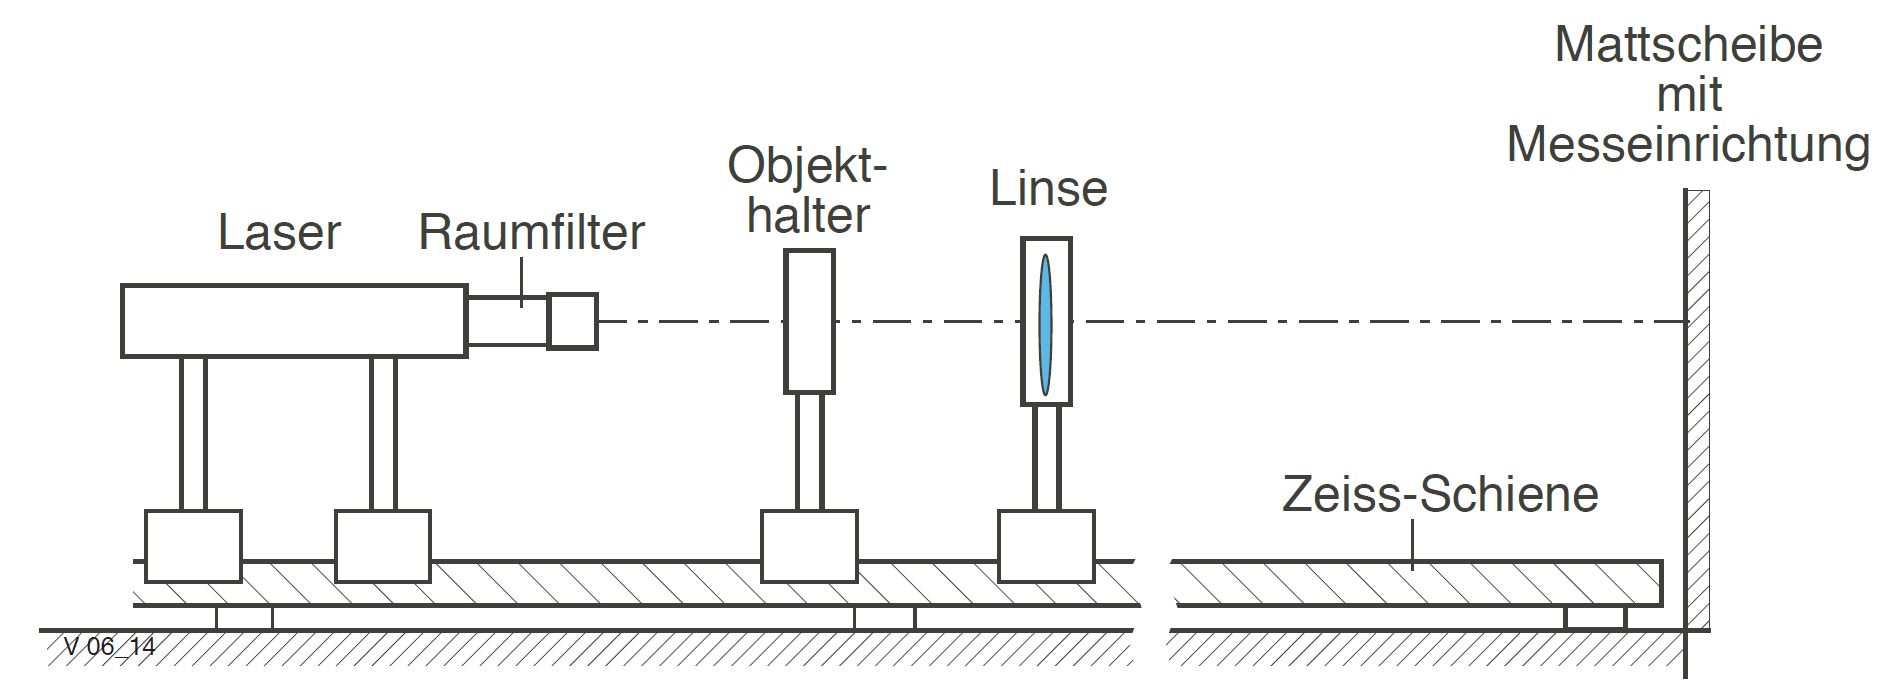
\includegraphics[width=\textwidth]{data/versuchsaufbau}
	\caption{Versuchsaufbau, des Laser, optische Elemente und der Mattscheibe}
	\label{fig:Versuchsaufbau}
\end{figure}

\begin{figure}[h!]
	\centering
	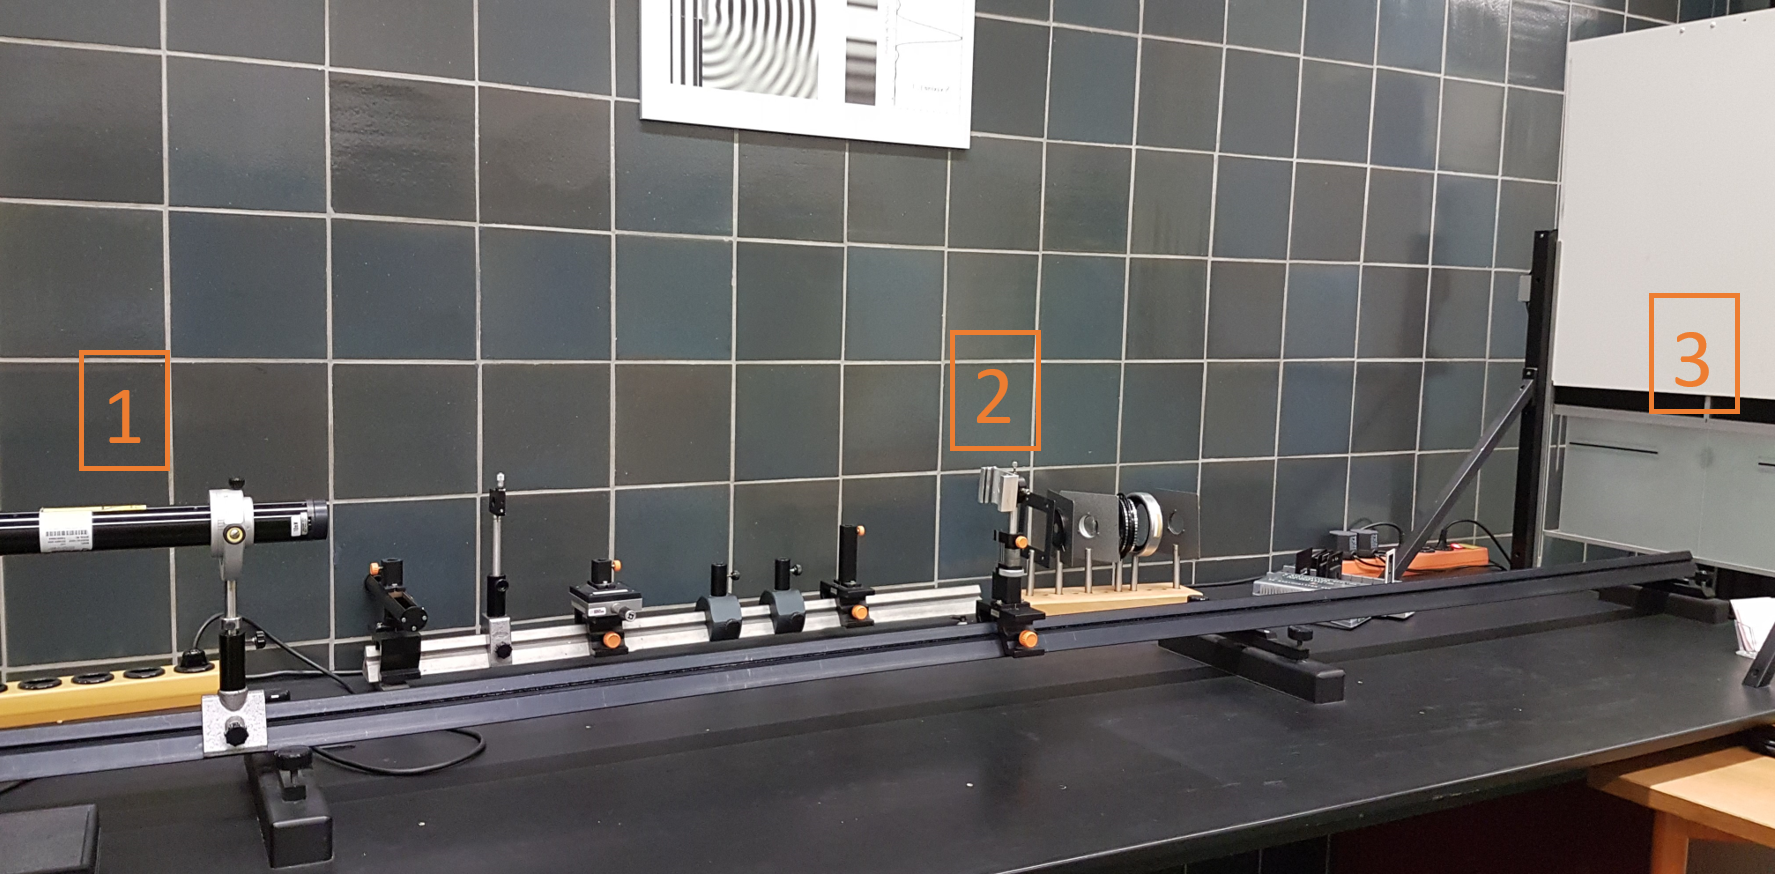
\includegraphics[width=\textwidth]{data/aufbau2}
	\caption{Versuchsaufbau mit dem Laser (1), mit dem Beugungsobjekt (2) und der Messeinrichtung (3).}
	\label{fig:org.Versuchsaufbau}
\end{figure}

% **************************************************************************** %
\subsection{Messmittel}
% **************************************************************************** %
\begin{table}[h!]
	\centering
	\begin{tabular}{|l|l|}
		\hline
		\rowcolor[rgb]{0.89,0.89,0.89}
		\textbf{Gerätebezeichnung} & \textbf{Typ}   \\ \hline
		Laser                      & He-Ne-Laser 632.8nm (rot)    \\ \hline
		Linse                      & f=2030mm                                     \\ \hline
	\end{tabular}
\caption{Messmittel die für den Versuchsaufbau genutzt wurden.}
\label{Messmittel}
\end{table}

% **************************************************************************** %
\subsection{Messobjekte}
% **************************************************************************** %
\begin{figure}[h!]
	\centering
	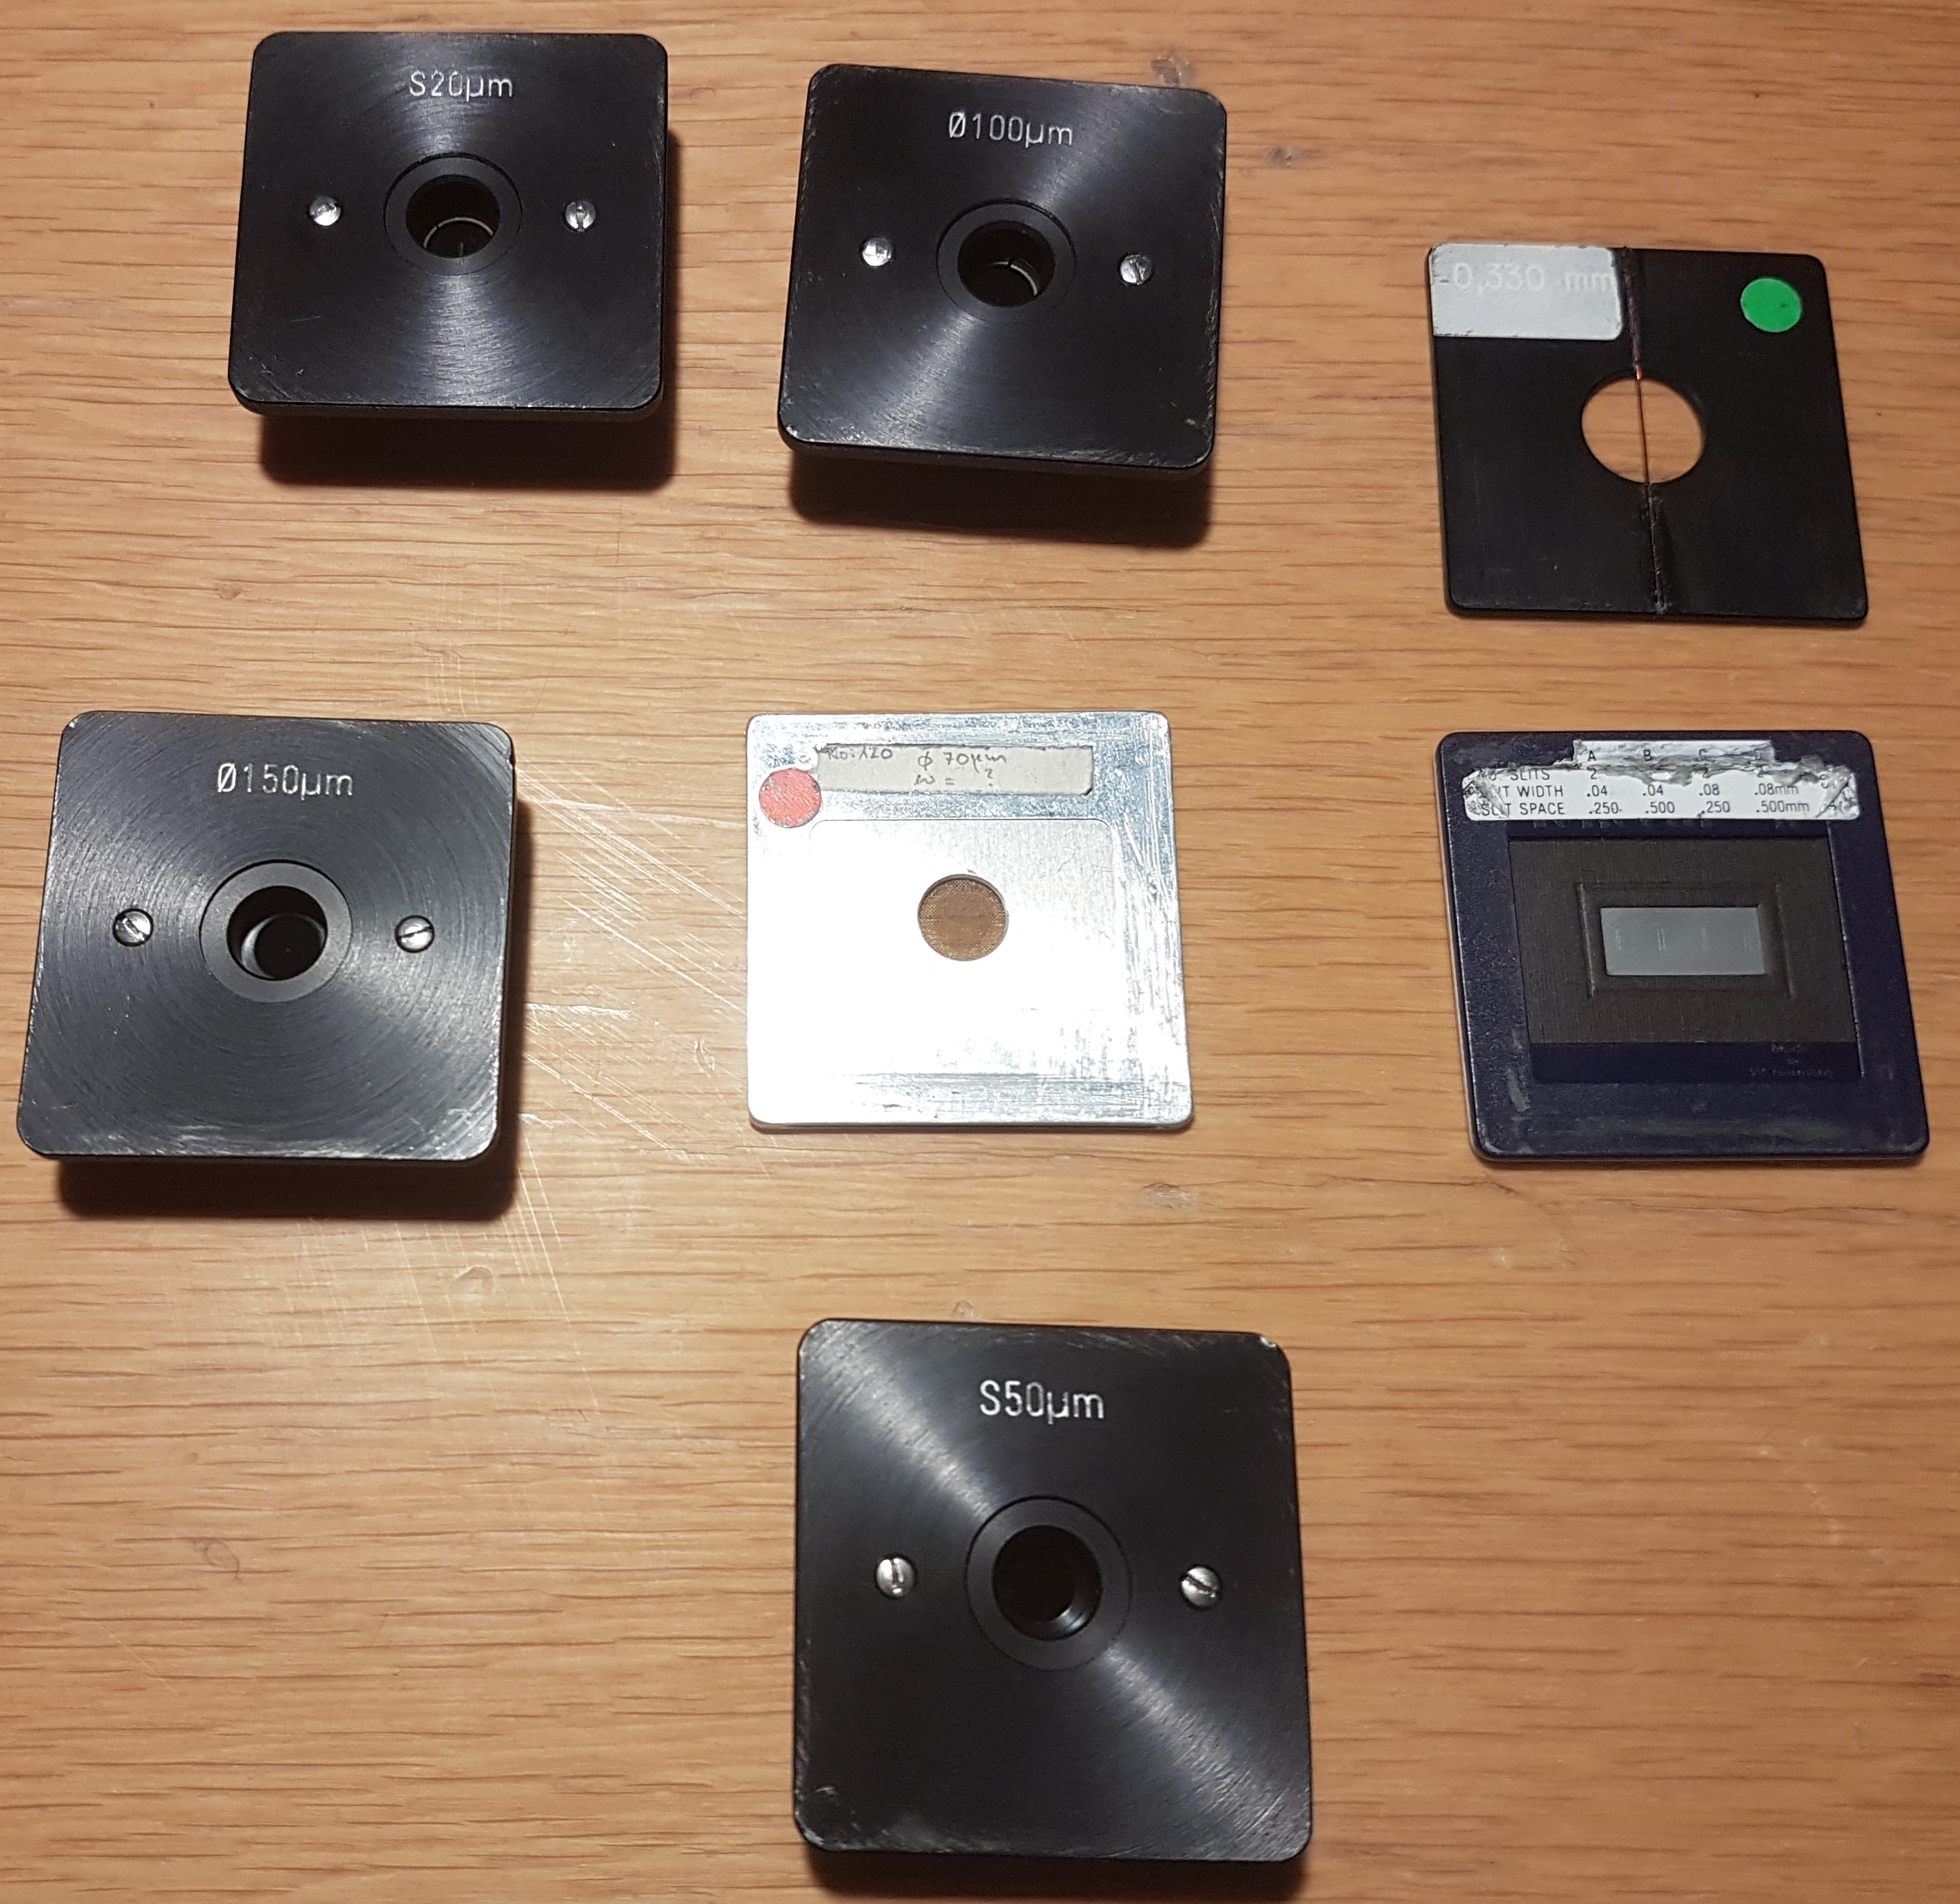
\includegraphics[width=0.6\textwidth]{data/objekte}
	\caption{Verschiedene Beugungsobjekt (Spalt, Antispalt, Loch, Gitter und Doppelspalt) die gemessen wurden}
	\label{fig:objekte}
\end{figure}

\begin{table}[h!]
	\centering
	\begin{tabular}{|l|l|}
		\hline
		\rowcolor[rgb]{0.89,0.89,0.89}
		\textbf{Typ} & \textbf{Breite}         \\ \hline
		Spalt 1      & 50    $ \cdot  10^{-6}m $    \\ \hline
		Spalt 2      & 200   $ \cdot  10^{-6}m $    \\ \hline
		Antispalt 1  & 0.33  $ \cdot  10^{-3}m $    \\ \hline
		Antispalt 2  & 0.124 $ \cdot  10^{-3}m $    \\ \hline
		Loch 1       & 150   $ \cdot  10^{-6}m $    \\ \hline
		Loch 2       & 100   $ \cdot  10^{-6}m $    \\ \hline
		Gitter       & 70    $ \cdot  10^{-6}m $    \\ \hline
		Doppelspalt  & 40    $ \cdot  10^{-6}m $    \\ \hline
	\end{tabular}
\caption{Messobjekte}
\label{table:messobjekte}
\end{table}
\newpage
% **************************************************************************** %
\subsection{Messvorgang}
% **************************************************************************** %
Bei diesem Versuch werden drei verschiedene Messungen durchgeführt. Diese Unterversuche sind:
\begin{itemize}
	\item Beugung am Spalt und Antispalt
	\item Beugung am Loch und Antiloch
	\item Beugung am Doppelspalt 
\end{itemize}

% **************************************************************************** %
\subsubsection{Beugung am Spalt und Antispalt}\label{cap:Spalt}
% **************************************************************************** %
Bei diesem Versuch werden die Abstände symmetrisch liegender Minima n-ter Ordnung bestimmt. Nach der Beugungstheorie mittels Regression kann aus diesen Werten die Breite des Spalts oder Drahtes berechnet werden. Dieser Messvorgang kann angewendet werden um den Durchmesser eines Haares oder einer Faser zu bestimmen.

\begin{figure}[h!]
	\centering
	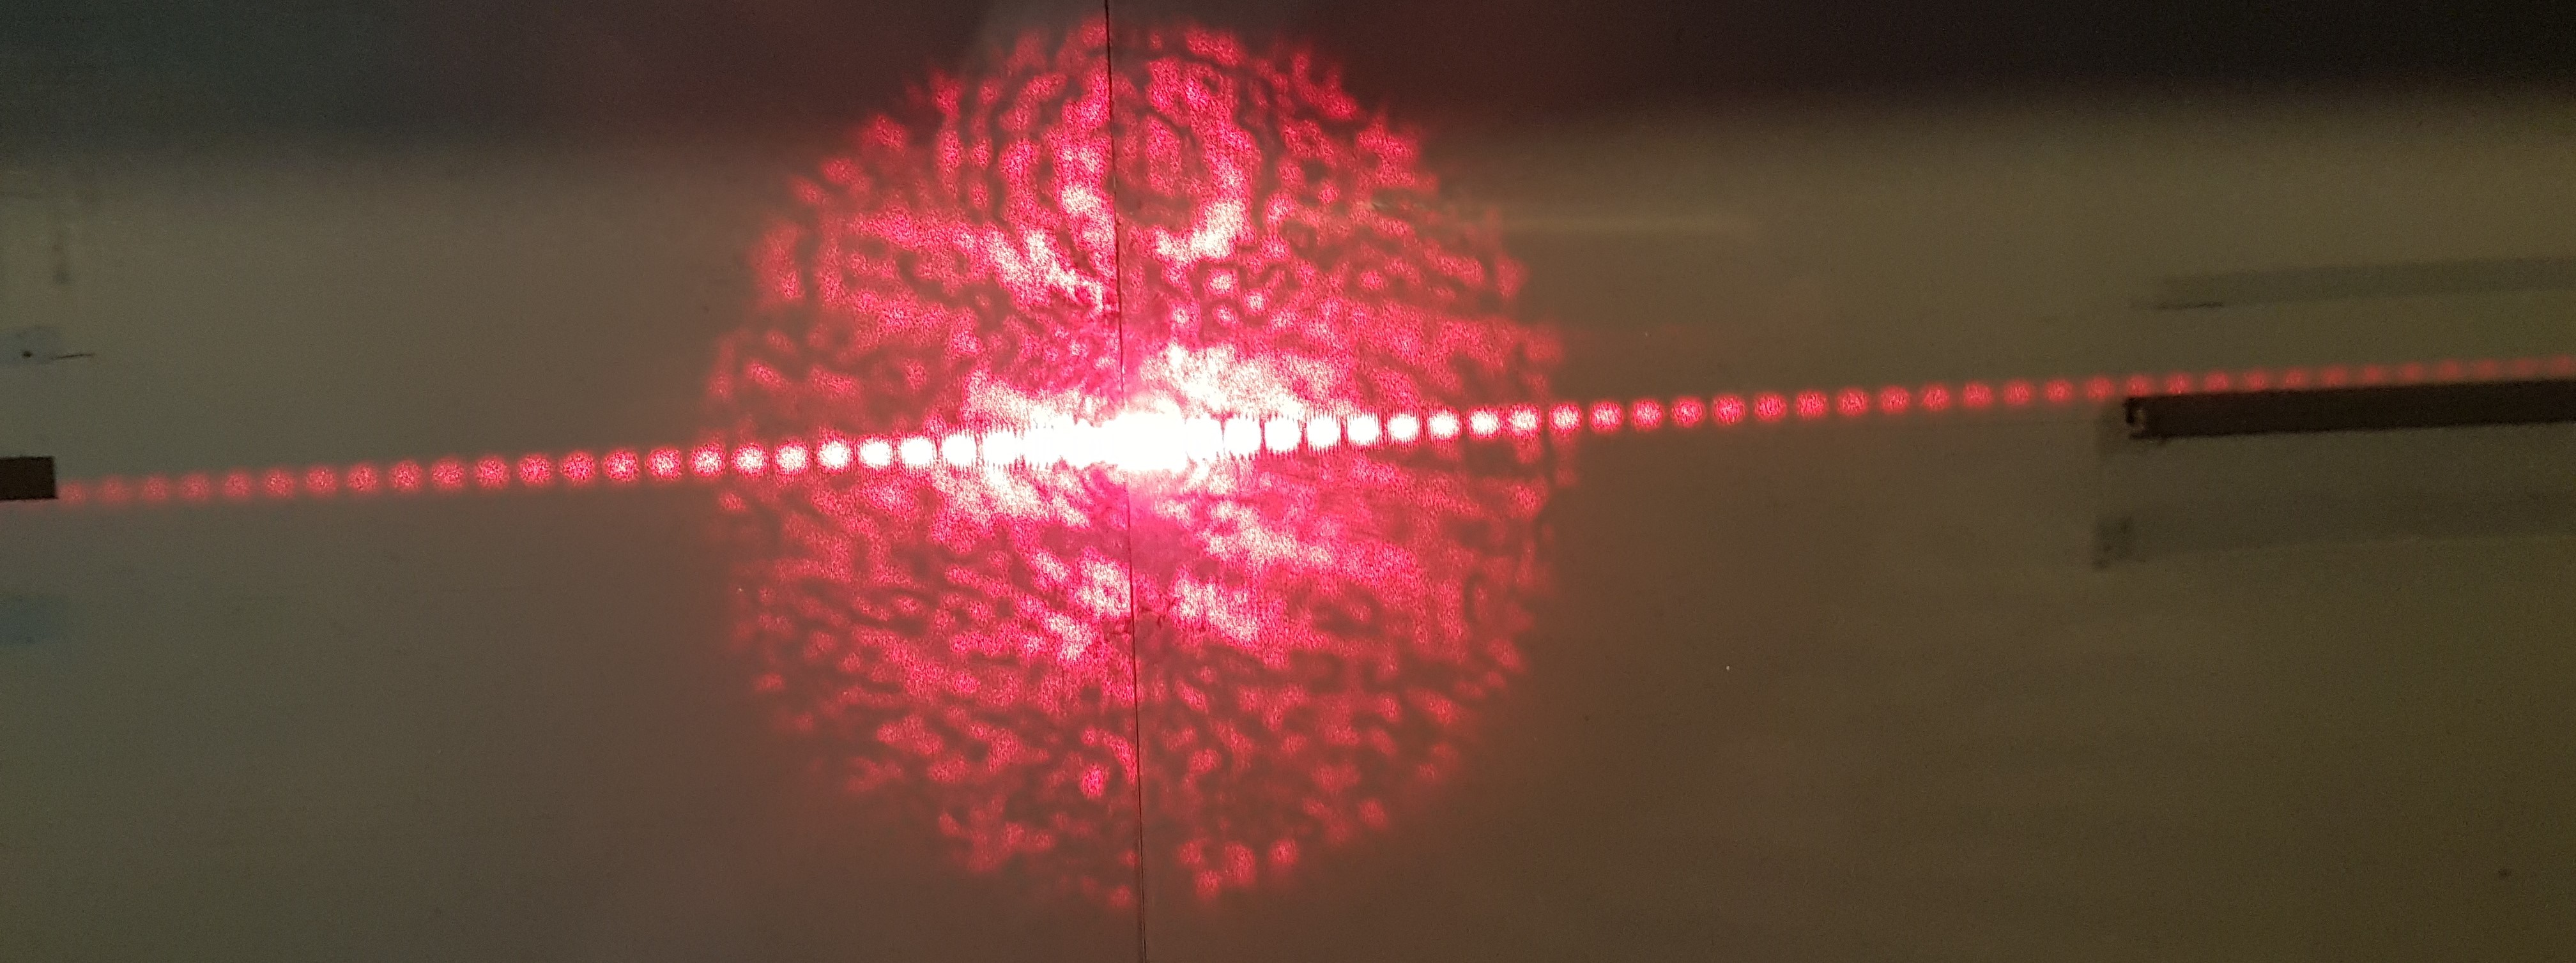
\includegraphics[width=0.5\textwidth]{data/versuch_spalt}
	\caption{Versuchsaufbau, des Laser, optische Elemente und der Mattscheibe}
	\label{fig:Versuchsaufbau}
\end{figure}

% **************************************************************************** %
\subsubsection{Beugung am Loch und Antiloch}
% **************************************************************************** %
Wie in dem Versuch \ref{cap:Spalt} wird anhand der beobachteten Minimas der Durchmesser des Loches bzw. mittleren Durchmesser der Teilchen berechnet. Wenn Pollenkörner untersucht werden, entsteht bei der Fraunhofer'scher Beobachtungsart dasselbe Interferenzmuster wie für ein einzelnes Objekt. In diesem Fall steigt die Intensität proportional zur Zahl der Beugungszentren an. Wenn sich verschiedene Interferenzmuster überlagern entsteht ein etwas verschwommenes Bild, welches dem mittleren Durchmesser entspricht.

\begin{figure}[h!]
	\centering
	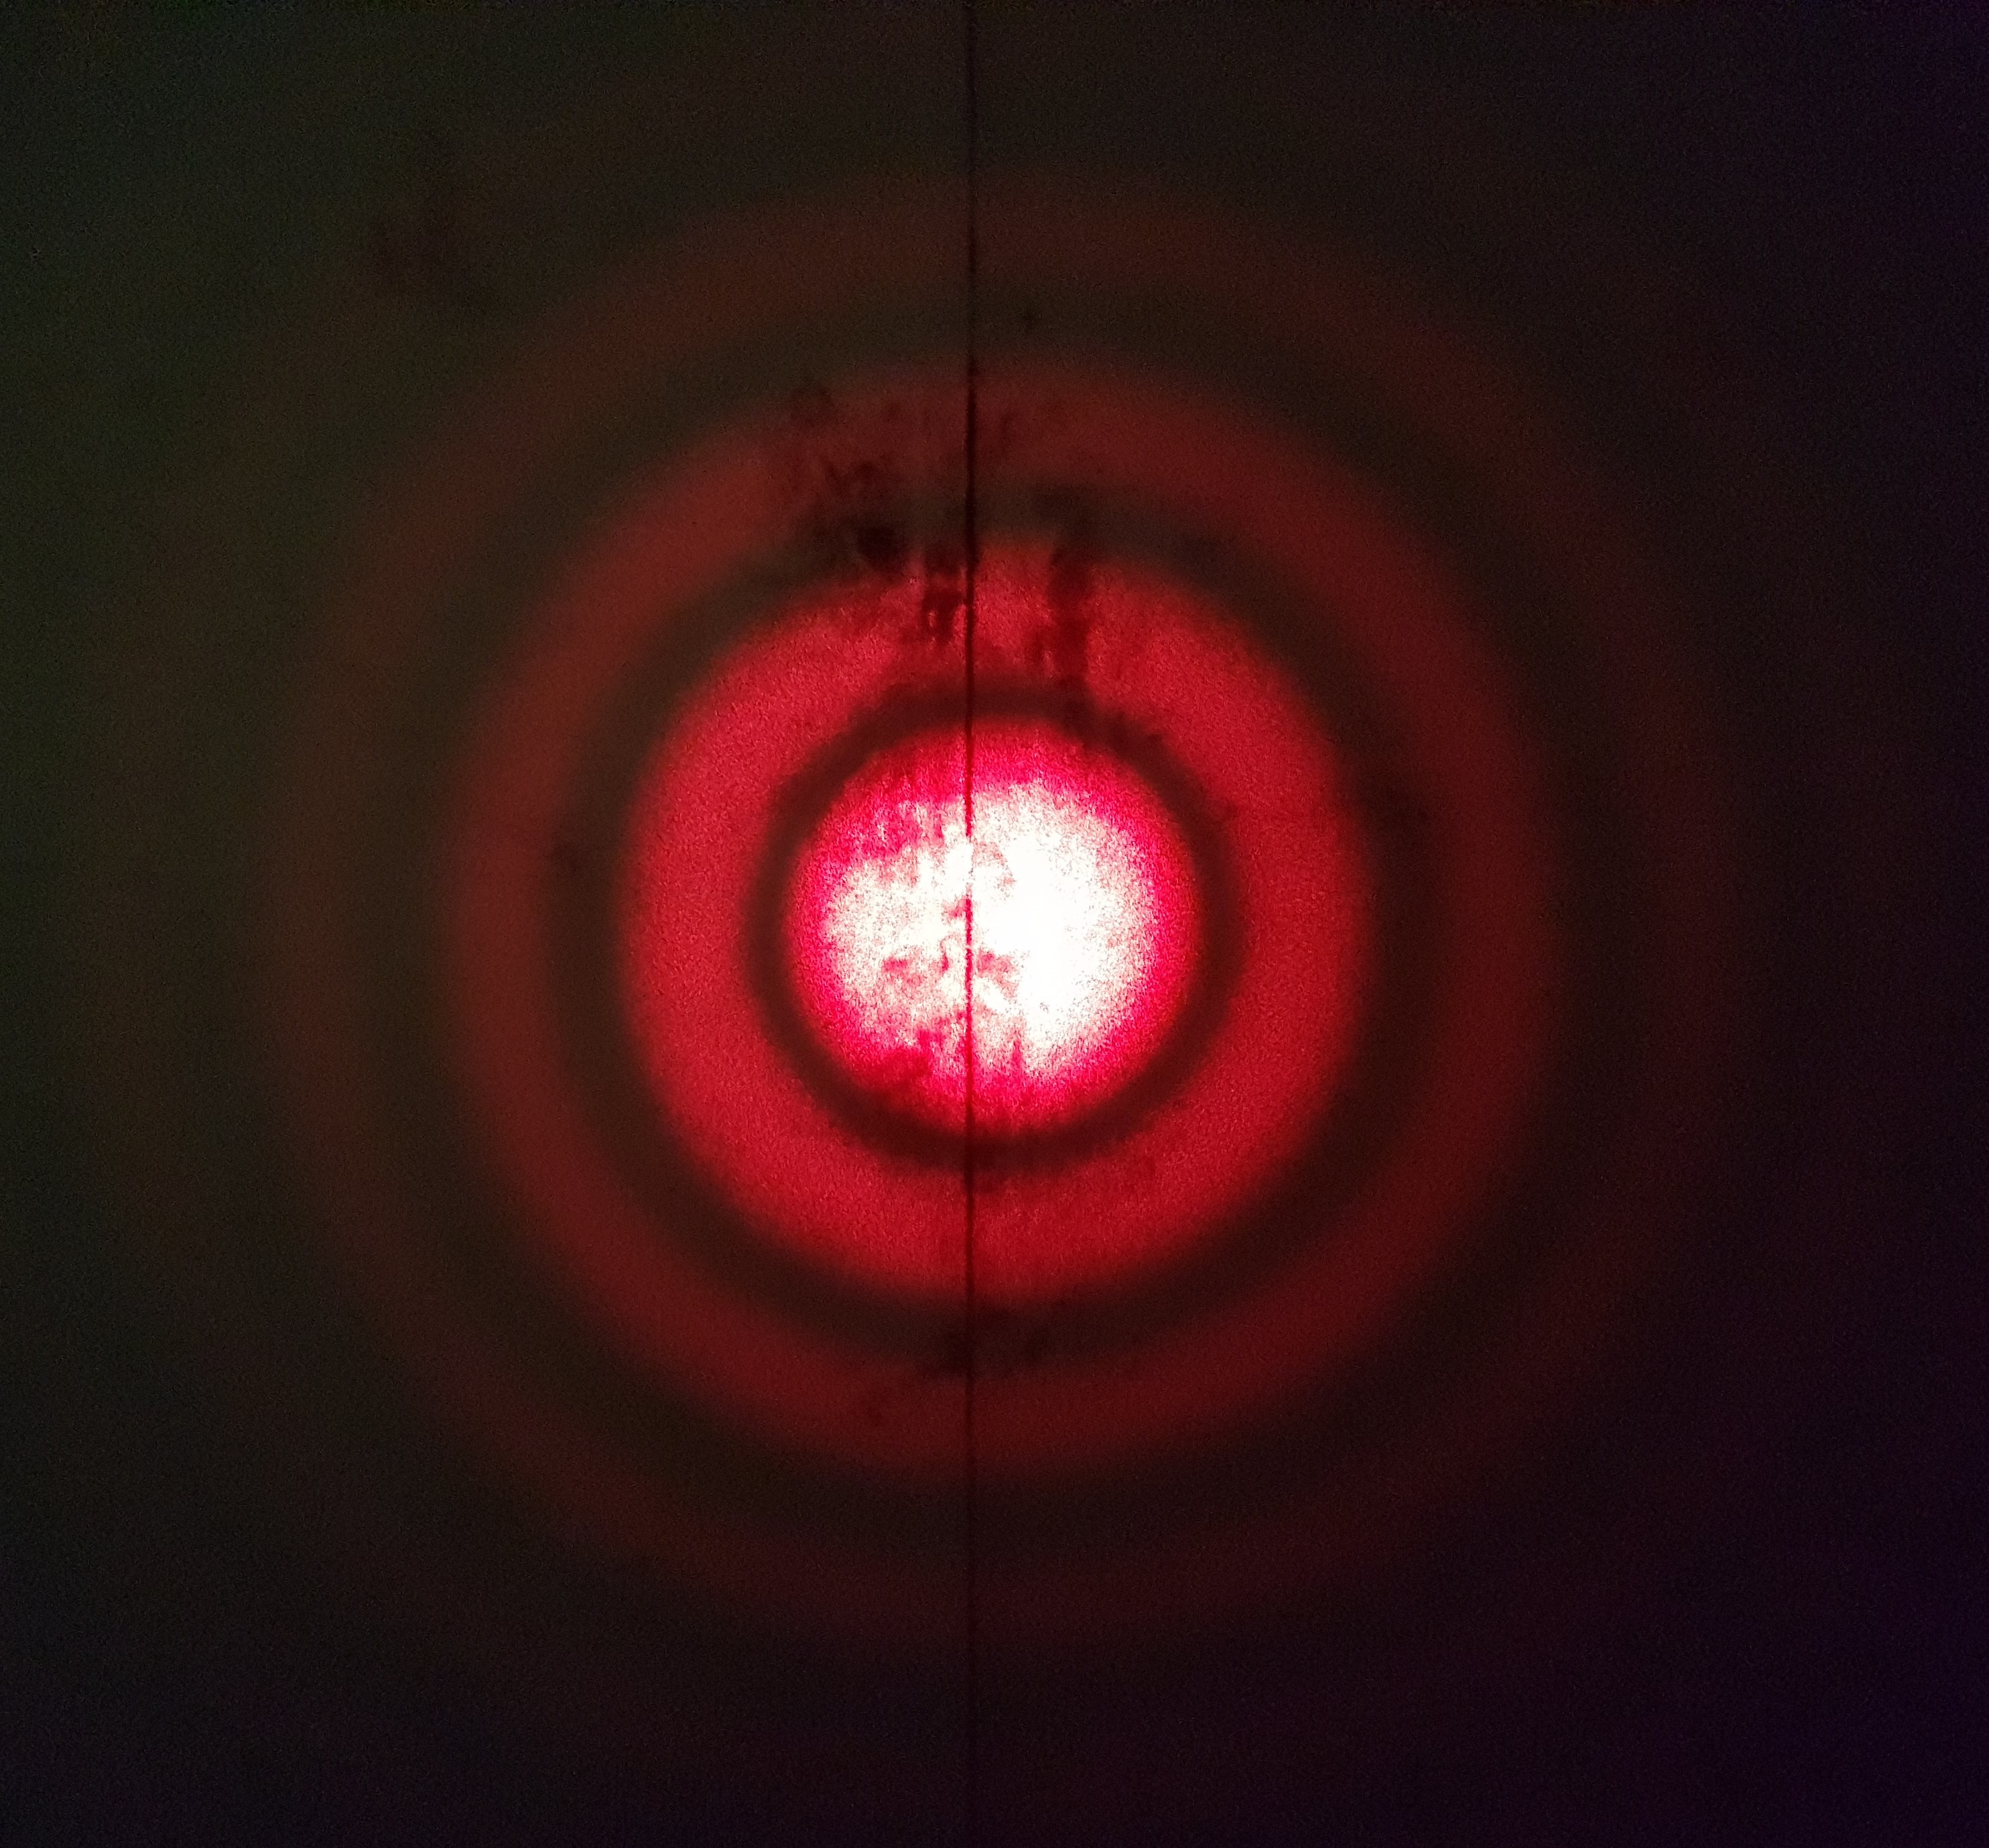
\includegraphics[width=0.5\textwidth]{data/versuch_loch}
	\caption{Versuchsaufbau, des Laser, optische Elemente und der Mattscheibe}
	\label{fig:Versuchsaufbau}
\end{figure}

% **************************************************************************** %
\subsubsection{Beugung am Doppelspalt}
% **************************************************************************** %

\newpage
% Kapitel 3----------------------------------------------------
% Kapitel 3 Auswertung-------------------------------------------------------- %
\section{Auswertung}
% ---------------------------------------------------------------------------- %


% **************************************************************************** %
\subsection{Beugung am Spalt und Antispalt}
% **************************************************************************** %

% **************************************************************************** %
\subsection{Beugung am Loch und Antiloch}
% **************************************************************************** %

% **************************************************************************** %
\subsection{Noch offen}
% **************************************************************************** %
\newpage
% Kapitel 4----------------------------------------------------
% Kapitel 1 Fehlerrechnung---------------------------------------------------- %
\section{Fehlerrechnung}
% ---------------------------------------------------------------------------- %

Die Fehlerrechnung für die wird anhand diesen Formel durchgeführt. Alle Berechnungen wurden in einem Matlabfile gerechnet, welches im Anhang hinterlegt ist.\\
Der Fehler bildet sich aus einem systematischen und einem statistischen Fehler.
 
% **************************************************************************** %
\subsection{Systematischer Fehler}
% **************************************************************************** %
Dieser Fehler $ s_{syst} $ besteht aus zwei Messfehler, welche die Messresultate beeinflussen. Diese Messfehler entstehen bei der Messung der Strecke zwischen zwei Minima des Interferenzmusters, sowie bei der Messung der Strecke von der Linse bis zum Schirm. Der Fehler $ s_{x} $ ist XXX und der Fehler $ s_{y} $ ist XXX. \\
Die Fehlerrechnung wurde mit folgender Formel durchgeführt. Dazu wurde die Formel \ref{} partiell abgeleitet.

\begin{equation}
s_{syst} = \sqrt{\left(\frac{\partial R}{\partial x}\cdot s_{x}\right)^2+\left(\frac{\partial R}{\partial y}\cdot s_{y}\right)^2}
\label{eq:syst Fehler}
\end{equation}

% **************************************************************************** %
\subsection{Statischer Fehler}
% **************************************************************************** %
Dieser Fehler kann direkt aus den Berechnungen von QtiPlot übernommen werden. In der Tabelle \ref{} ist der statische Fehler $ s_{stat} $ aufgeführt.

% **************************************************************************** %
\subsection{Gesamter Fehler}
% **************************************************************************** %
Mit der Geometrischen Addition kann der Gesamtfehler aus dem statischen und dem systematischen Fehler berechnet werden.

\begin{equation}
s_{tot} = \sqrt{(s_{sys})^2+(s_{stat})^2}
\label{eq:gesamter Fehler}
\end{equation}

Die Berechnungen wurden mit Matlab durchgeführt und das entsprechende File im Anhang hinterlegt. Die Resultate sind in der folgenden Tabelle \ref{} aufgeführt.
\newpage
% Kapitel 5----------------------------------------------------
\section{Resultate und Diskussion}\label{sec:diskussion}
Anfänglich wird hier eine allgemeine Tabelle präsentiert:

\begin{table}[H]
	\centering
	\begin{tabular}{ccc}
		Spalt $50\mu m$:		&  $49e-6$  	&  $\pm7e-7$\\
		Spalt $200\mu m$:		&  $196e-6$		&  $\pm6e-6$\\
		Antispalt $0.33mm$: 	&  $331e-6$		&  $\pm3e-6$\\
		Antispalt $0.124mm$:	&  $124e-6$		&  $\pm1e-6$\\
		Loch $150\mu m$: 		&  $69e-6$		&  $\pm4e-6$\\
		Loch $100\mu m$: 		&  $96e-6$		&  $\pm4e-6$\\
		Gitter $70\mu m$:  		&  $70e-6$		&  $\pm5e-6$\\
		Doppelspalt $40\mu m$: 	&  $616e-7$		&  $\pm5e-7$\\
	\end{tabular}
	\caption{Errechnete Endwerte}
	\label{tab:final}
\end{table}

\subsection*{Spalt $50\mu m$}
\begin{figure}[h!]
	\centering
	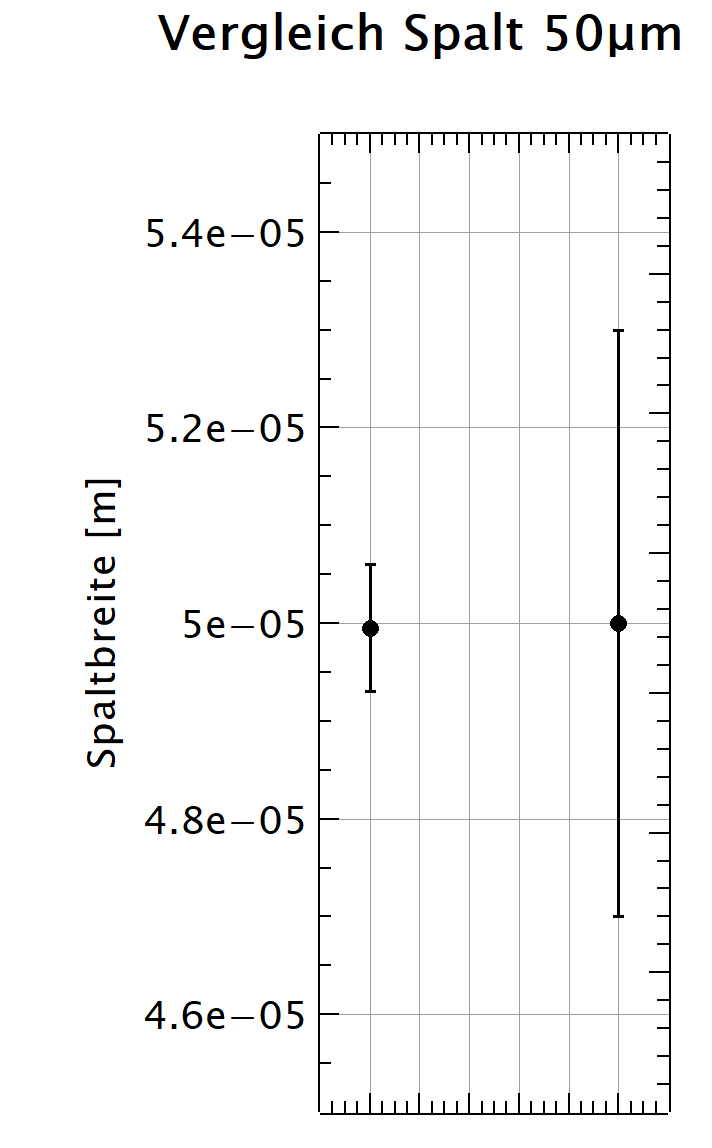
\includegraphics[width=0.4\textwidth]{data/dis_sp_50.png}
	\caption{Vergleich der gemessenen Werten mit den Theoretischen des $50\mu m$ Spalts}
	\label{fig:dis_spalt_50}
\end{figure}

\subsection*{Spalt $200\mu m$}
\begin{figure}[h!]
	\centering
	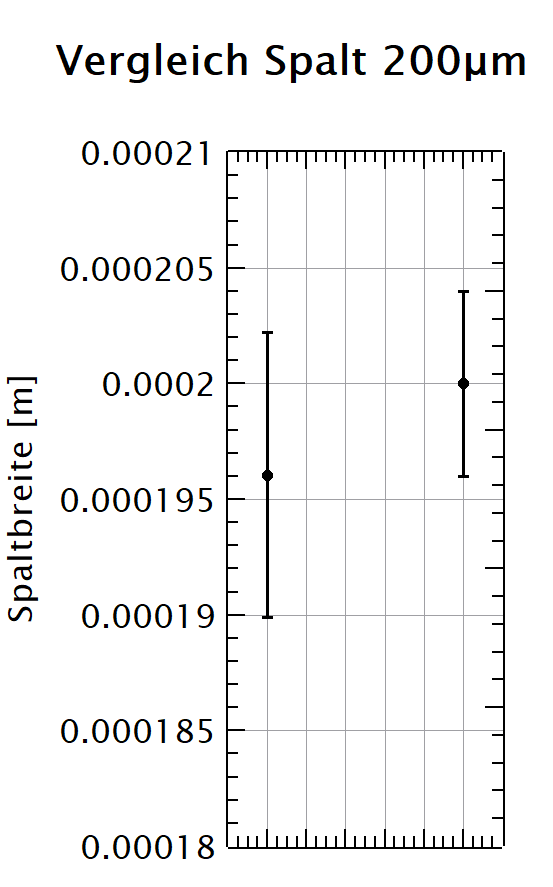
\includegraphics[width=0.4\textwidth]{data/dis_sp_200.png}
	\caption{Vergleich der gemessenen Werten mit den Theoretischen des $200\mu m$ Spalts}
	\label{fig:dis_spalt_200}
\end{figure}

\subsection*{Antispalt $0.33mm$}
\begin{figure}[h!]
	\centering
	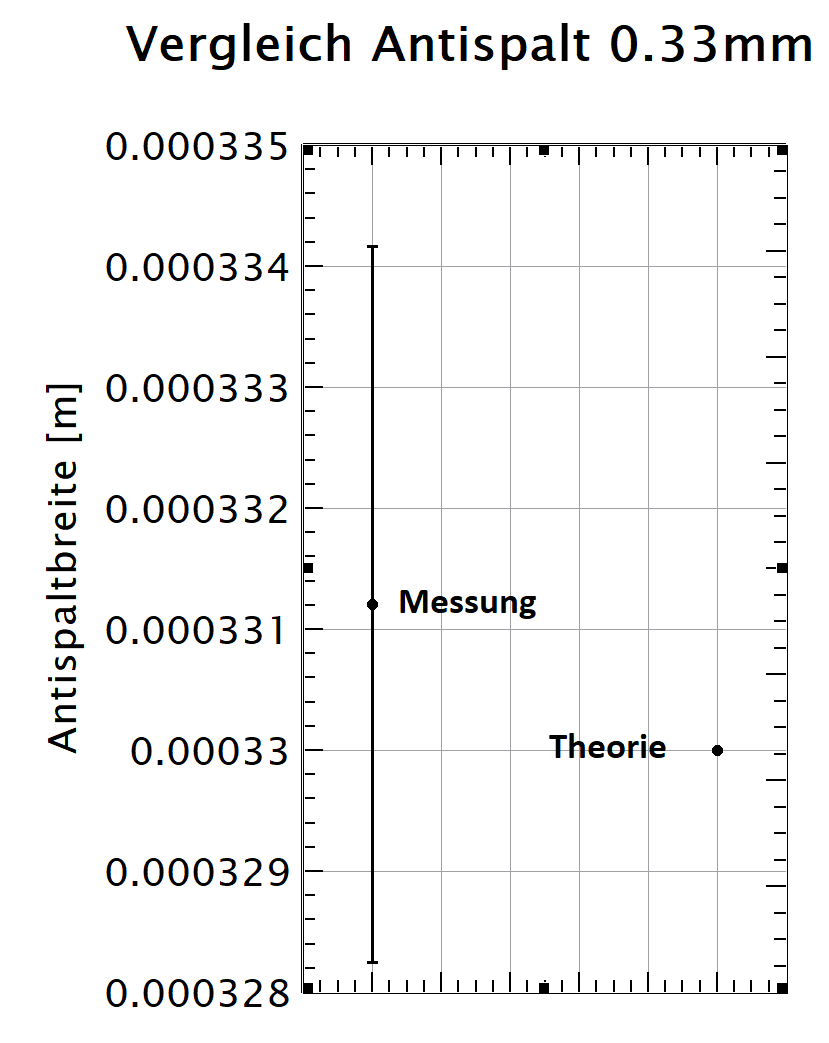
\includegraphics[width=0.4\textwidth]{data/dis_asp_33.png}
	\caption{Vergleich der gemessenen Werten mit den Theoretischen des $0.33mm$ Antispalts}
	\label{fig:dis_aspalt_33}
\end{figure}

\subsection*{Antispalt $0.124mm$}
\begin{figure}[h!]
	\centering
	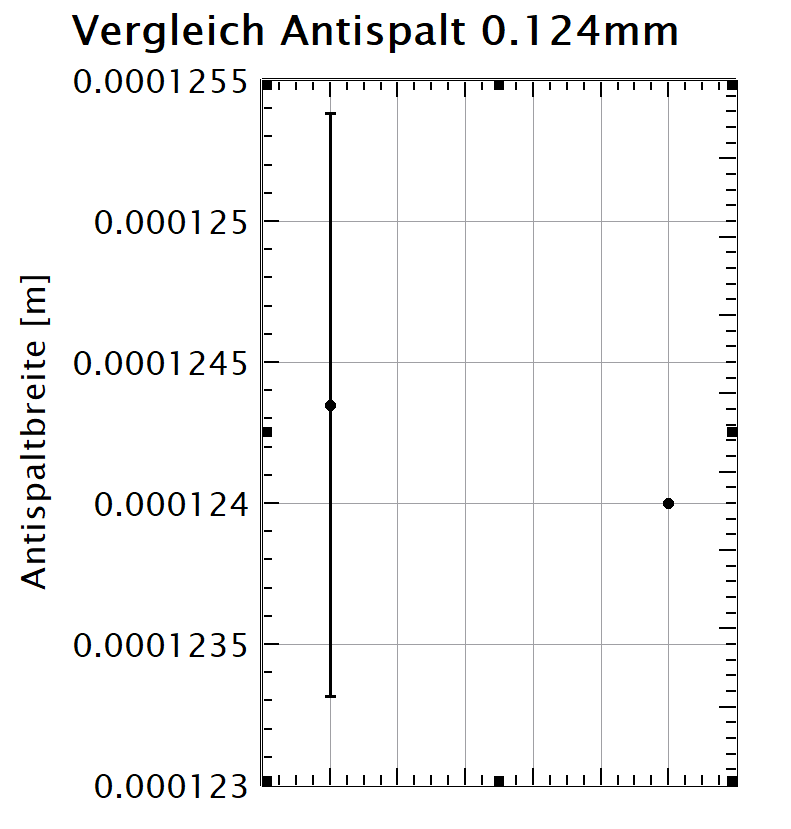
\includegraphics[width=0.4\textwidth]{data/dis_asp_12.png}
	\caption{Vergleich der gemessenen Werten mit den Theoretischen des $0.124mm$ Antispalts}
	\label{fig:dis_aspalt_12}
\end{figure}

\subsection*{Loch $150\mu m$}
\begin{figure}[h!]
	\centering
	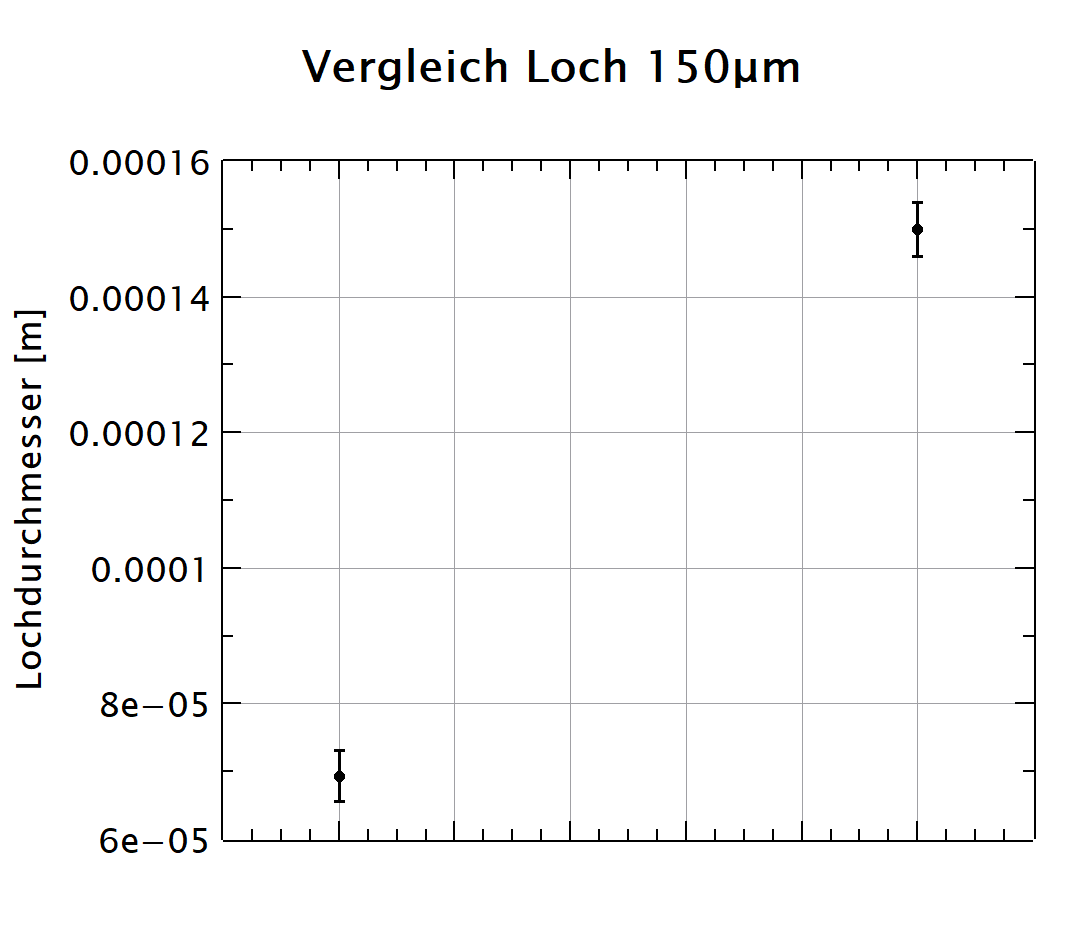
\includegraphics[width=0.4\textwidth]{data/dis_loch_150.png}
	\caption{Vergleich der gemessenen Werten mit den Theoretischen des $150\mu m$ Loch}
	\label{fig:dis_loch_150}
\end{figure}

\begin{figure}[h!]
	\centering
	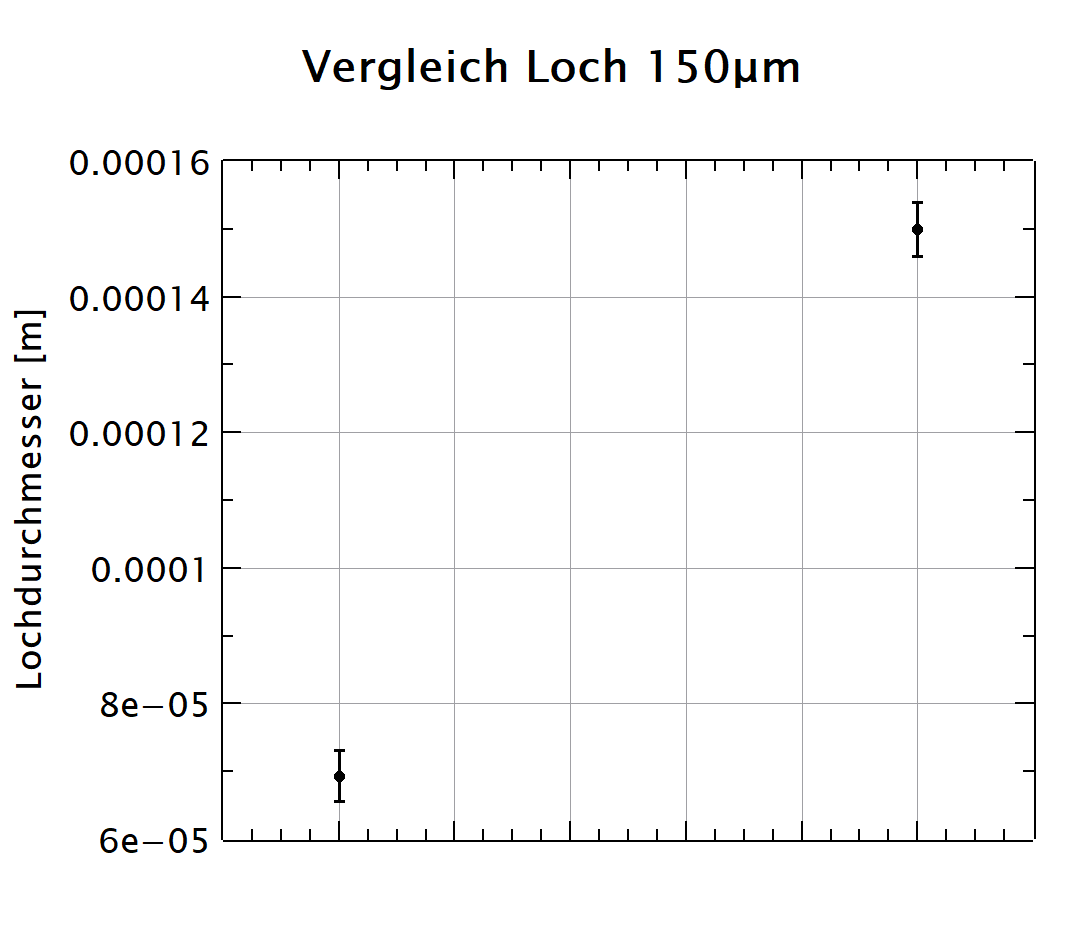
\includegraphics[width=0.4\textwidth]{data/dis_loch_150.png}
	\caption{Überprüfung des gemessenen Lochs mit Alternativer Messmethode}
	\label{fig:dis_loch_150}
\end{figure}

\subsection*{Loch $100\mu m$}
\begin{figure}[h!]
	\centering
	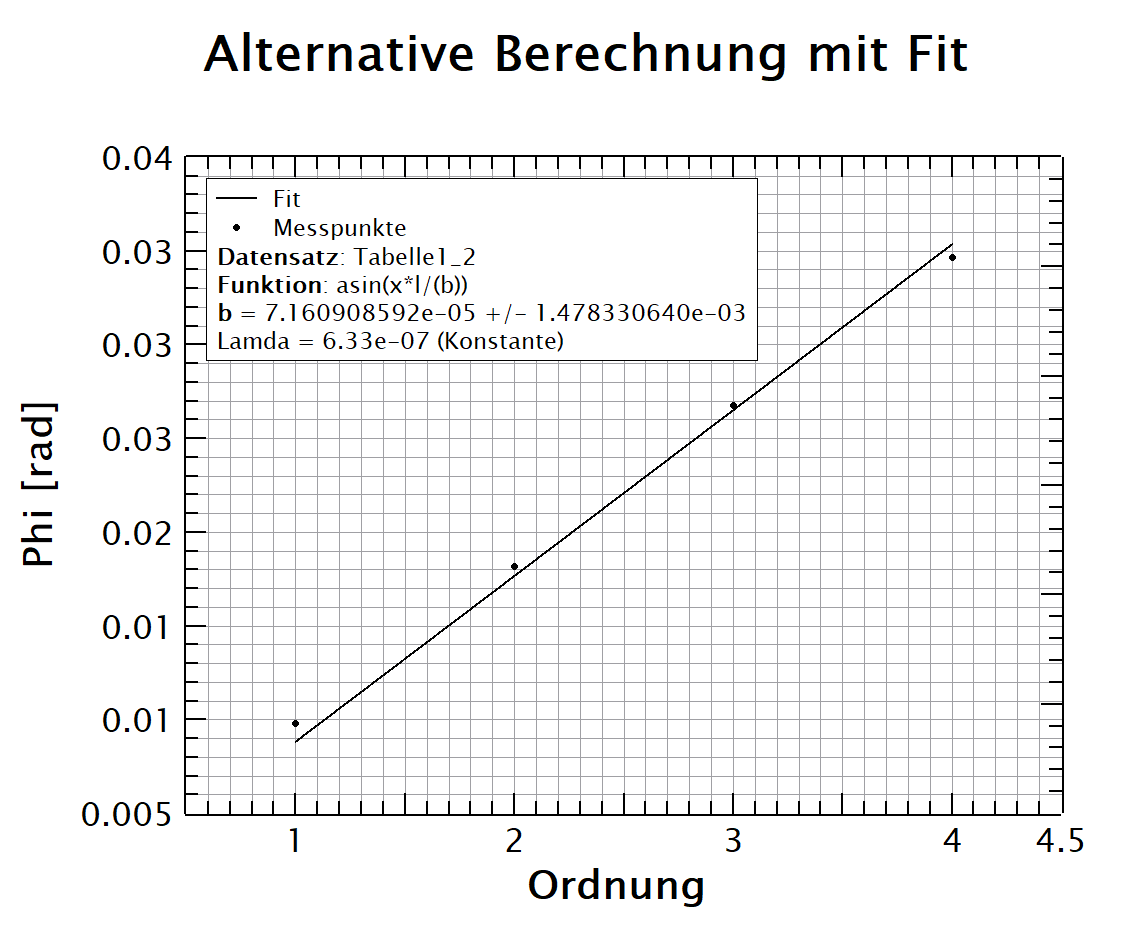
\includegraphics[width=0.4\textwidth]{data/fit_felerhaftes_loch.png}
	\caption{Vergleich der gemessenen Werten mit den Theoretischen des $100\mu m$ Loch}
	\label{fig:dis_loch_100}
\end{figure}

\subsection*{Gitter $70\mu m$}
\begin{figure}[h!]
	\centering
	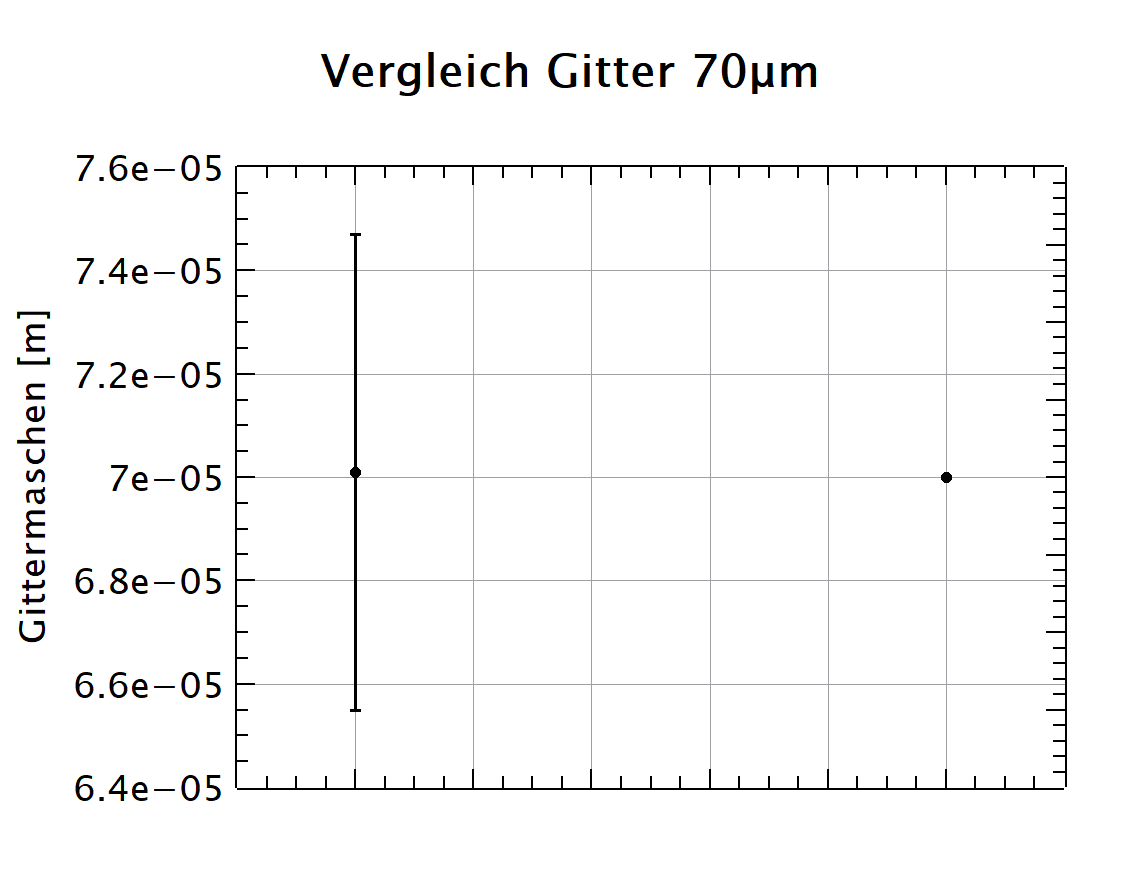
\includegraphics[width=0.4\textwidth]{data/dis_gitter.png}
	\caption{Vergleich der gemessenen Werten mit den Theoretischen des $70\mu m$ Gitter}
	\label{fig:dis_gitter}
\end{figure}

\subsection*{Doppelspalt $40\mu m$}
\begin{figure}[h!]
	\centering
	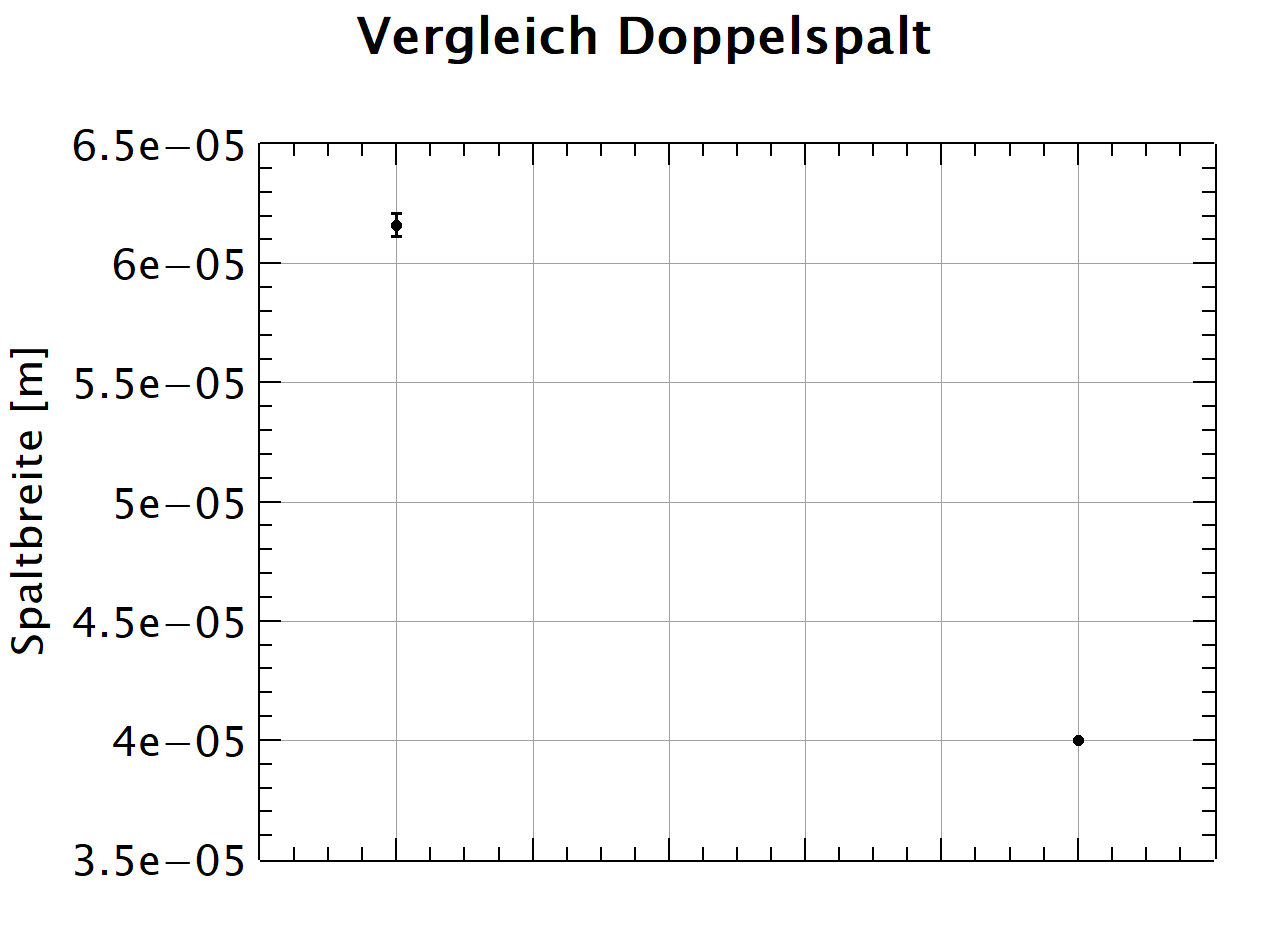
\includegraphics[width=0.4\textwidth]{data/dis_doppel.png}
	\caption{Vergleich der gemessenen Werten mit den Theoretischen des Wert Doppelspalts}
	\label{fig:Doppelspalt}
\end{figure}
\newpage


% Kapitel 6----------------------------------------------------
\section{Selbständigkeitserklärung}
% -------------------------------------------------------------
Mit meiner Unterschrift bestätige ich, dass ich das Laborheft selbständig verfasst habe.\\\\
Ort und Datum:\\\\
.................................................\\
Simon Zoller
\newpage


\begin{thebibliography}{xxxxxxxxxxxxxxxxxxx}
   \bibitem[BMBF, 2003]{bmbf}[1] Minamisawa, R. (22.10.2015). M1 Geschwindigkeit einer Pistolenkugel. 	 	   Windisch, FHNW.
   \bibitem[BMBF, 2003]{bmbf}[2]\,WaffenZimmi Bülach. (2017). http://www.waffenzimmi.ch/pressluftpistole-haemmerli-480-junior-p-4526.html.
\end{thebibliography}


\bibliography{literatur}

\listoffigures

\newpage 
% Kapitel 7----------------------------------------------------
\section{Anhang}
% -------------------------------------------------------------
Der Anhang wird per E-Mail an renato.minamisawa@fhnw.ch verdendet.
\begin{itemize}
	\item Excel-Tabelle $Pistolenversuch\_v1$
	\item Matlab-File $Fehlerrechnung$
\end{itemize}

\end{document}